\newcommand{\econtexRoot}{.}
% The \commands below are required to allow sharing of the same base code via Github between TeXLive on a local machine and ShareLaTeX.  This is an ugly solution to the requirement that custom LaTeX packages be accessible, and that ShareLaTeX seems to ignore symbolic links (even if they are relative links to valid locations)
\providecommand{\econtex}{\econtexRoot/texmf-local/tex/latex/econtex}
\providecommand{\econtexSetup}{\econtexRoot/texmf-local/tex/latex/econtexSetup}
\providecommand{\econtexShortcuts}{\econtexRoot/texmf-local/tex/latex/econtexShortcuts}
\providecommand{\econtexBibMake}{\econtexRoot/texmf-local/tex/latex/econtexBibMake}
\providecommand{\econtexBibStyle}{\econtexRoot/texmf-local/bibtex/bst/econtex}
\providecommand{\notes}{\econtexRoot/texmf-local/tex/latex/handout}
\providecommand{\handoutSetup}{\econtexRoot/texmf-local/tex/latex/handoutSetup}
\providecommand{\handoutShortcuts}{\econtexRoot/texmf-local/tex/latex/handoutShortcuts}
\providecommand{\handoutBibMake}{\econtexRoot/texmf-local/tex/latex/handoutBibMake}
\providecommand{\handoutBibStyle}{\econtexRoot/texmf-local/bibtex/bst/handout}

  
\documentclass[titlepage]{\econtex}\newcommand{\texname}{ConsumptionHeterogeneity}
\usepackage{\econtexSetup}\usepackage{\econtexShortcuts}
%\usepackage[nolists,nomarkers,tablesonly]{endfloat}
\usepackage{tikz}
\usepackage{caption}
\usepackage{titlesec}
\setcounter{secnumdepth}{4}
\usepackage{placeins}
\usepackage{pdfpages}
\usepackage{setspace}
\usepackage{breqn}
\onehalfspacing

\usepackage{booktabs,rotating}

\titleformat{\paragraph}
{\sffamily\mdseries\normalsize}{\theparagraph}{1em}{}
\titlespacing*{\paragraph}
{0pt}{3.25ex plus 1ex minus .2ex}{1.5ex plus .2ex}



\begin{document}\bibliographystyle{\econtexBibStyle}
\input Switches.tex

\begin{verbatimwrite}{\jobname.title}
Monetary Policy Transmission with Many Agents
\end{verbatimwrite}

%\hfill{\tiny \jobname}

\title{ 
	\bigskip
	\bigskip
	Monetary Policy Transmission \\ with Many Agents}

\author{
  Edmund Crawley\authNum   \\ {\small JHU}
  \and
  Seungcheol Lee\authNum    \\ {\small UCL}
}


\keywords{}
\jelclass{}

\date{March 2019}
\maketitle


\begin{abstract}
We analyze the transmission mechanism of monetary policy to consumption in New Keynesian models with heterogeneous agents. We show that in these models the countercyclical nature of profits, empirically false, plays a large role in amplifying the intertemporal substitution channel. On the other hand the interest rate exposure channel, empirically large, plays a small role. Our analysis makes use of the partial equilibrium decomposition of \cite{auclert_monetary_2017} which we show to perform well even in models where the assumptions do not hold. We suggest expanding the role of the interest rate exposure channel, while dampening the amplification effect of countercyclical profits, is of primary quantitative importance in future work.
\end{abstract}


\begin{authorsinfo}
\name{Crawley: Department of Economics, Johns Hopkins University, \href{mailto:ecrawle2@jhu.edu}{\texttt{ecrawle2@jhu.edu}}}
\name{Lee: University College London, \href{mailto:seungcheol.lee@ucl.ac.uk}{\texttt{seungcheol.lee@ucl.ac.uk}}}
\end{authorsinfo}

\titlepagefinish
\setcounter{page}{1}

\pagebreak
\section{Introduction}
What is the mechanism via which a monetary policy shock affects consumption? In standard representative agent New Keynesian (RANK) models this is through the intertemporal substitution channel: when real interest rates decline, the price of consumption today drops relative to the price in the future, so households choose to consume more today.

However, recent evidence from microdata has brought this mechanism into question.\footnote{In particular household marginal propensity to consume appear to be much higher than RANK models would suggest (e.g. \cite{parker_consumer_2013} among many others) and the elasticity of intertermporal substitution is likely small (e.g. \cite{best_estimating_2018})} A number of new models claim to match both the micro and macro data better.

This paper uses the lens of the monetary policy decomposition presented in \cite{auclert_monetary_2017} to analyze some standard modeling approaches. The advantage of Auclert's decomposition is that it can be very closely tied to the microdata.  However, strictly it requires assumptions that do not hold up in many models. Our paper also analyzes how useful the decomposition is in these cases. In particular the method assumes that a transitory monetary policy shock has no persistent effects.  This is clearly the case in any model with no predetermined variables: transitory shocks cannot be propagated into the future because there are no state variables that can carry information with them. Such models include the standard RANK model without capital as well as the beseline two agent New Keynesian (TANK) model we consider in this paper. We break this assumption in two ways. First, we add capital, a predetermined variable, to our TANK model which results in persistence of a monetary policy shock due to the slow movement of the capital stock. Second, in our heterogeneous agent New Keynesian (HANK) model, the entire distribution of assets is a predetermined state variable with potentially important dynamics.

\subsection{Findings}
We begin our analysis with a standard TANK model in which a proportion of households live hand-to-mouth, have no debt, and earn only labor income.\footnote{We closely follow \cite{dgHANKTANK} here.} As there is no debt neither the interest rate exposure not the Fisher channel play a role. We find instead a large role being played by the earnings heterogeneity channel: firm profits are countercyclical in the New Keynesian model, so the poor households see significantly more income variation over the business cycle than the wealthy. This is an important finding and draws into question some of the key results in the HANK literature so far. That profits are countercyclical is not empirically true, so this transmission mechanism does not fit the evidence.\footnote{\cite{broer_2018} come to a similar conclusion.}

Without a large earnings heterogeneity channel, the standard TANK model would continue to lean very heavily on the intertemporal substitution channel. Our next iteration of the model shows a potential for a very different transmission mechanism, one that fits the microdata but that current models do not quantitatively capture. We allow the hand-to-mouth households in our TANK model to maintain a debt up to some fraction of their steady state income. When interest rates are low they will be able borrow a little more, and when they are high a little less, thus providing an interest rate exposure channel through which monetary policy acts.

We find the income channels (both aggregate and heterogeneous) act as a multiplier for both the intertemporal substitution and the interest rate exposure channels. As we decrease the elasticity of intertemporal substitution, the intertemporal substitution channels diminishes along with the income multipliers of it. The interest rate exposure channel, on the other hand, remains the same size. This suggests it may be possible to create a monetary policy model in which intertemporal substitution plays no role at all, but which nonetheless fits the macrodata. This is something we plan to tackle in future work.

The rest of the paper investigates how useful Auclert's decomposition is in models with predetermined variables. Our first such model extends the  TANK model with capital. We find the decomposition fails when we have no convex capital adjustment costs, but that with standard parameterizations of these costs the decomposition accounts for over 95 percent of the change in consumption.

Finally we consider a one-asset HANK model.\footnote{Our model closely relates to the two asset model presented in \cite{blSolving}.} This breaks with the assumption required for Auclert's decomposition in two ways. First, as with other HANK models the entire distribution of assets is a predetermined state variable, allowing for potential persistence following a monetary policy shock. Second, its use of Greenwood-Hercowitz-Huffman (GHH) non-separable preferences introduces a sixth transmission mechanism relating to the Hicksian elasticity of consumption with hours worked. We show that although the distribution of assets is predetermined, a monetary policy shock has little persistence. However, the strong link between consumption and hours worked in the GHH preference specification acts as a large transmission mechanism, and one for which there is little empirical support. We conclude that GHH preferences should not be used in quantitative models of this kind.\footnote{For a related detailed criticism of GHH preferences, see \cite{arGHH}.}

Overall we believe significant progress has been made in understanding the transmission mechanism of monetary policy recently, both empirically and theoretically. However, we find there is still a great deal of divergence between the two and believe going forward models should target the interest rate exposure and aggregate income channels, and give the intertemporal substitution and earnings heterogeneity channel as smaller role.

\section{Transmission Channels} \label{transmission_channels}
We will make heavy use of the monetary policy partial equilibrium decomposition described in \cite{auclert_monetary_2017}. He makes the assumption that for an individual a one time shock to nominal interest rates looks like i) a transitory change in income, ii) a one off change in the price level, iii) a change in the real interest rate. Here we provide a brief description of each of the five channels he identifies and then give some indication as to the conditions under which they sum to the aggregate change in consumption. For more detail please refer to Auclert's paper.

\subsection{Aggregate Income Channel}
The aggregate income channel measures how much consumption changes due to the change in aggregate income, under the assumption that all incomes move proportionally. The size of this channel is given by:
\begin{align}
\textit{AggInc} = \mathbb{E}_i \left( \text{MPC}_i Y_i  \right) \frac{dY}{Y}
\end{align}
where $\text{MPC}_i$ is the marginal propensity to consume of household $i$ and the expectation is taken over all households.\footnote{Strictly this is the marginal propensity to consume out of income \textit{after} accounting for labor response. In our models hours are either rationed or do not depend on wealth, so this definition of MPC coincides with the more standard definition.} That is the aggregate income channel is the income weighted marginal propensity to consume multiplied by the change in aggregate income.

\subsection{Earnings Heterogeneity Channel}
A monetary policy shock may not change the income of every household proportionally. If households with high MPCs see relatively larger income changes than households with low MPCs, then overall the channel through which monetary policy affects consumption through income will be larger than measured by the aggregate income channel. The total income channel is simply the expectation of each household's MPC multiplied by their own change in income, $\mathbb{E}_i \left( \text{MPC}_i dY_i  \right) $. The earnings heterogeneity channel is measured as the residual of the total income channel after taking away the aggregate income channel:
\begin{align}
\textit{EarnHet} = \mathbb{E}_i \left( \text{MPC}_i dY_i  \right) - \mathbb{E}_i \left( \text{MPC}_i Y_i  \right) \frac{dY}{Y}
\end{align}

\subsection{Interest Rate Exposure Channel}
The interest rate exposure channel measures how much households change their consumption due to unhedged interest rate exposure (URE). Unhedged interest rate exposure is defined as the difference between all maturing assets (including income) and maturing liabilities (including planned consumption), and is therefore the quantity of saving that is planned to be invested at this periods interest rate. When this period's real interest rate goes up, this effectively increases the budget constraint of those households who have positive unhedged interest rate exposure. Under certain conditions these households will increase their consumption by their MPC multiplied by the change in their budget constraint. That is:
\begin{align}
\textit{IRE} = \mathbb{E}_i \left( \text{MPC}_i \text{URE}_i  \right) \frac{dR}{R}
\end{align}
where $R$ is the real interest rate.

\subsection{Fisher Channel}
Inflation has the effect of changing the real value of nominal assets and debts. The Fisher channel measures how this affects aggregate consumption, making the assumption that households individual MPCs apply to this change in wealth. The key household level measure here is the net nominal position (NNP), that is the sum of all nominal assets net of nominal debts for each household. The size of the channel is then:
\begin{align}
\textit{Fisher} = -\mathbb{E}_i \left( \text{MPC}_i \text{NNP}_i  \right) \frac{dP}{P}
\end{align}
where $P$ is the price level.

\subsection{Intertemporal Substitution Channel}
Finally the intertemporal substitution channel measures how much households will shift their consumption between time periods due to the change in the real interest rate.
\begin{align}
\textit{IntSubs} = \mathbb{E}_i \left( \frac{1}{\sigma_i} (1-\text{MPC}_i) \frac{C_i}{C}  \right) \frac{dR}{R}
\end{align}
where $\frac{1}{\sigma_i}$ is the household's elasticity of intertemporal substitution, $C_i$ is their consumption this period and $C$ is the mean level of consumption this period.

\subsection{Aggregation}
\cite{auclert_monetary_2017} shows the conditions under which these five channels sum exactly to the aggregate change in consumption following a monetary policy shock. First, preferences must be separable. Second, a monetary policy shock has a purely transitory effect, changing income and the real interest rate for one period only, while effecting a one time change in the price level. For New Keynesian models with no predetermined variables, such as the standard consumption New Keynesian model or the baseline two agent New Keynesian model presented below, this is the case. Models with capital, or where the distribution of wealth persists into the next period such as the HANK model presented below, do not fit this decomposition. We will measure the error as the difference between the sum of the five channels and the actual change in consumption.


\section{A TANK Model in which the Decomposition Work Exactly}

\subsection{Model Overview}
We begin our analysis with a baseline two agent New Keynesian (TANK) model. Our baseline TANK model is composed of two types of agents, Ricardian and Keynesian, along with a continuum of intermediate goods firms, a perfectly competitive final goods firm, and a monetary policy authority. The model is closely related to the standard New Keynesian model with Calvo pricing frictions, the main difference being the addition of the Keynesian households. A key addition in our model, compared with other TANK models, is to allow for the Keynesian households to hold a non-zero quantity of short term nominal debt (owed to the Ricardian households) so that we have non-trivial levels for households' unhedged interest rate exposure (URE) and net nominal positions (NNP).

The advantage of starting our analysis with this model is that it contains no predetermined variables, and therefore the conditions for our partial equilibrium decomposition hold exactly. As well as being a useful starting point to build upon, it also highlights how the transmission mechanism works in TANK models (and HANK models more generally), highlighting just how important the earnings heterogeneity channel is in these models.

\subsection{Households}
A proportion $\lambda$ of households, which we shall call Keynesian, live hand-to-mouth, consuming all their income in each period. The remaining ($1-\lambda$), which we shall call Ricardian, are unconstrained optimizing agents. Following \cite{dgHANKTANK}, and in order to keep the supply side as simple as possible, we assume the markup on wages (see below) is high enough that households supply as much labor as demanded by the firms.

\subsubsection{Ricardian Households}
Each period Ricardian households choose how much to consume, $C^R_t$, in order to maximize their life time (separable) utility:
\begin{align*}
\mathbb{E}\sum_{t=0}^{\infty}\beta^t \left(\frac{\left(C^R_t\right)^{1-\sigma}}{1-\sigma} - \frac{\left(N^R_t\right)^{1+\psi}}{1+\psi}\right)
\end{align*}
where $N^R_t$ is their hours worked. They are subject to the budget constraint:
\begin{align*}
P_t C^R_t + I_{t}^{-1}B_{t+1} =  N^R_t W_t + P_t D_t + B_t
\end{align*}
where $P_t$ is the price level in period $t$, $I_t$ is the gross nominal interest rate between $t$ and $t+1$, $B_t$ is the quantity of bonds bought at time $t-1$ paying one unit of nominal currency in period $t$, $W_t$ is the nominal wage per unit of labor in period $t$ and $D_t$ is the real dividend payed by firms in period $t$. All firm profit goes to the Ricardian households and this is shared equally between them.

The Euler equation for these Ricardian households IS:
\begin{align}
%\frac{W_t}{P_t} = \left(C^R_t\right)^{\sigma}\left(N^R_t\right)^{\psi} \label{foc_hours_R} \\
\left(C^R_t\right)^{-\sigma} = \beta \mathbb{E}\left(I_t\frac{P_{t}}{P_{t+1}} \left(C^R_{t+1}\right)^{-\sigma}\right)	\label{euler_R}
\end{align}

\subsubsection{Keynesian Households}
Keynesian households are more impatient that the Ricardian households and as a result are up against their borrowing limit. They can borrow nominal bonds up to the point where their expected \textit{real} payment in the next period is equal to a fixed fraction $\Omega$ of their steady state income. Each period they optimize their period utility:
\begin{align*}
\frac{\left(C^K_t\right)^{1-\sigma}}{1-\sigma} - \frac{\left(N^K_t\right)^{1+\psi}}{1+\psi}\
\end{align*}
subject to their budget constraint:
\begin{align}
C^K_t \leq N^K_t \frac{W_t}{P_t} + \left(I_{t}^{-1} \frac{\mathbb{E}_t P_{t+1}}{P_t} -  \frac{\mathbb{E}_{t-1}P_t }{P_t}\right)\Omega \bar{N_K}\overline{W/P}  \label{budget_constraint_K}
\end{align}
where $\overline{W/P}$ and $\bar{N_K}$ are the steady state real wage and hours worked by Keynesian households.

%Their first order condition for consumption and labor is:
%\begin{align}
%\frac{W_t}{P_t} = \left(C^K_t\right)^{\sigma}\left(N^K_t\right)^{\psi} \label{foc_hours_K}
%\end{align}

\subsubsection{Household Aggregation and Wage Schedule}
With the Keynesian proportion of households equal to $\lambda$, total consumption is:
\begin{align}
C_t = \lambda C^K_t + (1-\lambda) C^R_t \label{agg_C}
\end{align}
Hours are equally rationed between both types of household such that:
\begin{align}
N_t = N^K_t = N^R_t	\label{agg_N}
\end{align}
The real wage is set according to the demand schedule:
\begin{align}
\frac{W_t}{P_t} = \mathcal{M}^{\omega} \left(C_t\right)^{\sigma}\left(N_t\right)^{\psi} \label{foc_hours}
\end{align}
where $\mathcal{M}^{\omega}>1$ can be interpreted as the gross average markup of wages. We assume $\frac{W_t}{P_t} \geq \left(C^R_t\right)^{\sigma}\left(N^R_t\right)^{\psi} \geq \left(C^K_t\right)^{\sigma}\left(N^K_t\right)^{\psi}$ so that households always provide the hours demanded by the firms.\footnote{This demand schedule follows \cite{dgHANKTANK} and is close to the wages a union representing both types of household would set. We also tried allowing wages to be set by the market. This results in counter-factual results such as Keynesian and Ricardian households moving their hours worked in opposite directions during a recession.}

\subsection {Firms}
The production side of the economy follows the standard New Keynesian model with Calvo price adjustment. The firm side of the economy is identical to that presented in \cite{gali_book} except for the fact that firms choose both labor and capital (and thus their production function has constant returns to scale) each period. This simplifies the analysis a little, as all firms share the same marginal cost. In our base model we hold the aggregate quantity of capital constant, but including it here allows for easy extension to the model with investment.

\subsubsection{Final Goods Firm}
The final goods firm produces a final consumption good, $Y_t$, from intermediated inputs, $X_t(j)$ for $j \in [0,1]$ using the technology:
\begin{align*}
Y_t = \left( \int_0^1 X_t(j)^{1-\frac{1}{\varepsilon}} dj \right)^{\frac{\varepsilon}{\varepsilon-1}}
\end{align*}
Profit maximization yields the demand schedule $X_t(j) = \left(\frac{P_t(j)}{P_t}\right)^{-\varepsilon}$ where $P_t$ is the price of the final good. Competition also imposes a zero profit condition that yields $P_t = \left(\int_0^1 P_t^{1-\varepsilon}\right)^{\frac{1}{1-\varepsilon}}$.

\subsubsection{Intermediate Goods Firm}
There is a continuum of intermediate goods firms, indexed by $j \in [0,1]$ each of which uses both labor and capital each period according to the production function:
\begin{align*}
X_t(j) = A K_t(j)^\alpha N_t(j)^{1-\alpha}
\end{align*}
As our focus is on monetary policy shocks, we assume the technology level ($A$) to be constant. Constant returns to scale results in the marginal cost being equal for all firms.

The probability that a firm is able to adjust its price in any period is equal to $1-\theta$. A firm that is able to adjust its price in period $t$ will choose a price $P^*$ to maximize the current market value of profits it will make while the price remains effective. That is firm $j$ solves the problem:
\begin{align}
\underset{P^*}{\max} \sum_{k=0}^{\infty} \theta^k \mathbb{E}_t \{{\Lambda}_{t,t+k} X_{t+k}(j) (P_t^* - MC_{t+k}P_{t+k}) \} \label{profit_max}
\end{align}
subject to the demand constraints:
\begin{align}
X_t(j) = \left(\frac{P_t^*}{P_{t+k}}\right)^{-\varepsilon} \label{demand_constraint}
\end{align}
where ${\Lambda}_{t,t+k} = \beta^k \left(\frac{c^R_{t+k}}{c^R_{t}}\right)^{-\sigma} \left( \frac{P_t}{P_{t+k}} \right)$ is the stochastic discount factor for nominal payoffs, for the Ricardian households who own the profits from the firms. 

The first order condition arising from \ref{profit_max}  and \ref{demand_constraint} is:
\begin{align}
\sum_{k=0}^{\infty} \theta^k \mathbb{E}_t \Big\{{\Lambda}_{t,t+k} X_{t+k}(j) \left(P_t^* - \frac{\varepsilon}{\varepsilon-1}MC_{t+k} P_{t+k}\right)  \Big\} = 0 \label{foc_pricing}
\end{align}

Finally, with only a fraction $1-\theta$ of firms changing their prices in any given period, the aggregate price level moves according to:
\begin{align*}
P_t = \left(   \theta P_{t-1}^{1-\varepsilon} + (1-\theta)(P_t^*)^{1-\varepsilon}\right)^{\frac{1}{1-\varepsilon}}
\end{align*}

\subsection{Monetary Policy}
We assume the central bank follows a simple log-linear Taylor rule with weight on inflation only:
\begin{align}
i_t = \phi_{\pi} \pi_t + \nu_t	\label{taylor_rule}
\end{align}
where $i_t$ and $\pi_t$ are the log deviations from the nominal steady-state interest rate and inflation rate respectively. In line with the transitory nature of the experiment we are running, we assume no persistence in $\nu_t$.

\subsection{Equilibrium}
As our baseline model has no investment, the goods market clearing condition is:
\begin{align}
Y_t = C_t	\label{agg_prod}
\end{align}
and the total capital and labor used must equal that available, $\int_0^1 K_t(j)dj = \bar{K}$ and $\int_0^1 N_t(j)dj = N_t$.

\subsection{Steady State}
We will study small fluctuations around the zero inflation steady-state. As hours are allocated evenly between the two types of households we have that the share of hours worked by Keynesians is $\overline{n}_{K} = \lambda$, and that by Ricardians is $\overline{n}_{R} = 1-\lambda$. The steady state consumption shares ($\overline{c}_{K} = \lambda\overline{C^K}/\overline{Y}$ and $\overline{c}_{R} = \lambda\overline{C^R}/\overline{Y}$) are less simple, both because Ricardians earn all the income from the firms and they get paid interest from the Keynesian households' debt. In steady-state the markup over marginal cost is equal to $\frac{\varepsilon}{\varepsilon-1}$, and the real wage is equal to the marginal productivity of labor adjusted down by this markup, $(1-\alpha) \frac{\varepsilon-1}{\varepsilon}\frac{\overline{Y}}{\overline{N}}$. 

Using this steady-state wage, along with the Keynesian budget constraint (\ref{budget_constraint_K}) we can identify the steady-state ratio of Keynesian consumption:
\begin{align}
\overline{c}_{K} = \lambda \left(1-\Omega(1-\beta)\right)\frac{\varepsilon-1}{\varepsilon}(1-\alpha) \label{c_K_ss}
\end{align}

\subsection{Log-linearized Model}
We use small letters to indicate percentage changes from steady-state values and then linearize around the steady-state. We begin with the basic building blocks of the New Keynesian model. First the Euler equation for Ricardian households, linearized from equation \ref{euler_R}, becomes:
\begin{align}
c^R_t = \mathbb{E}_t c^R_{t+1} - \frac{1}{\sigma}(i_t - \mathbb{E}_t\pi_{t+1}) \label{euler_R_linear}
\end{align}
The New Keynesian Phillips curve, derived from the pricing equation \ref{foc_pricing}, is:
\begin{align}
\pi_t=\beta \mathbb{E}_t\pi_{t+1}+\frac{(1-\theta)(1-\beta\theta)}{\theta}\left(\sigma +  \frac{\psi + \alpha}{1-\alpha} \right)\tilde{y}_t \label{NKphillips_linear}
\end{align}
where the output gap, $\tilde{y}_t$, in this case with fixed technology and capital is just the percentage deviation of output from steady-state output.

The monetary policy rule is already linearized and we take it directly from equation \ref{taylor_rule}.

Unlike the standard New Keynesian model, these three are not enough to pin down the model as the Euler equation (\ref{euler_R_linear}) is determined by Ricardian households, while total consumption and production involves the Keynesians too. We have the aggregation conditions from equations \ref{agg_C}, \ref{agg_N} and \ref{agg_prod}:
\begin{align}
c_t &= \overline{c}_{K} c^K_t + \overline{c}_{R} c^R_t \label{agg_C_linear} \\
n_t &= \overline{n}_{K} n^K_t + \overline{n}_{R} n^R_t \label{agg_N_linear} \\
\tilde{y}_t &= c_t \label{agg_prod_linear}
\end{align}
and the Keynesian budget condition from equation \ref{budget_constraint_K}:
\begin{align}
(1-\Omega (1-\beta)) c^K_t = w_t + n^K_t + \Omega \left(\pi_t - \mathbb{E}_{t-1}\pi_t\right) - \beta \Omega  (i_t - \mathbb{E}_t \pi_{t+1})  \label{budget_constraint_K_linear}
\end{align}
where $w_t$ is the real wage in period $t$. Note $\pi_t - \mathbb{E}_{t-1}\pi_t$ represents unexpected inflation between $t-1$ and $t$ and relates to the net nominal position of the Keynesian households. The expected return on nominal bonds, $r_t = i_t - \mathbb{E}_t \pi_{t+1}$, would be the real interest between $t$ and $t+1$ if such a market existed and relates to the unhedged interest rate exposure of the Keynesian households. In the case where there is no debt ($\Omega=0$), both these components of the budget constraint disappear. Further note that in this model $\mathbb{E}_{t-1}\pi_t$ will always be equal to zero, so the model has no predetermined variables.

The first order condition for hours worked, equation \ref{foc_hours}, along with the equal allocation of hours, give:
\begin{align}
w_t &= \sigma c_t + \psi n_t \label{foc_hours_linear} \\
n^R_t &= n^K_t
\end{align}
Finally the connection between hours worked and the output gap is given by:
\begin{align}
\tilde{y}_t &= (1-\alpha)n_t  \label{production_linear}
\end{align}
Note capital does not appear in the linearized production function because of the fixed capital assumption.

The final baseline model consists of the Taylor rule, equation \ref{taylor_rule}, along with the equations \ref{euler_R_linear} through \ref{production_linear} and the identity $r_t = i_t - \mathbb{E}_t \pi_{t+1}$.

\subsection{Calibration}
We calibrate to standard parameters based on annual periods. Baseline parameters are shown in table \ref{table:calibration}. We will vary some of these to see how the size of the different transmission mechanisms changes with them.

\input ../Matlab/DynareCode//Tables/calib_table.tex

\section{Results from the Baseline TANK Model}
As there are no predetermined variables in our baseline TANK model the decomposition of transmission mechanisms described in section \ref{transmission_channels} works exactly. Here we look at how monetary policy divides into the five different channels according to the proportion of Keynesian households, as well as the extent to which they are able to take on debt.

\subsection{Model with No Debt}
To start we consider the model in which the Keynesian households cannot hold any debt, as is standard in TANK models.\footnote{For examples see \cite{dgHANKTANK}, \cite{gali_understanding_2007} and \cite{broer_2018}.} The transitory nature of the shock means that expected inflation next period is zero, and hence a one percent decrease in the nominal rate translate exactly into a one percent decrease in the real rate (if it were to trade).

Figure \ref{fig:ProportionKeynesian} shows the size of each transmission channel following a one percentage point decrease in the nominal interest rate, where the proportion of Keynesian households is on the x-axis. Note that both the interest rate exposure channel and the Fisher channel are absent in this model as there is no debt between the two types of agent. The left side of the graph shows the transmission channels when there are very few Keynesian households. As has been well documented\footnote{e.g. \cite{kaplan_monetary_2016}} the intertemporal substitution model dominates in this case, seen here in the division of transmission channels along the y-axis corresponding to the RANK model. We have set the elasticity of intertemporal substitution equal to one, so a one percentage point decrease in the real interest rate increases consumption of the Ricardian households by exactly one percent. This is seen as the intercept with the y-axis, divided into a large intertemporal substitution channel of size $\beta$, and a small aggregate income channel of size $1-\beta$.

Moving along the x-axis increases the proportion of Keynesian households. The size of the intertemporal substitution channel decreases in line with the consumption share of consumption by Ricardian households. As Ricardian households own all the capital as well as the profits from the firms, their consumption share falls more slowly that their share of households. As we introduce Keynesian households the size of the aggregate income channel increases, as the average MPC across households grows. While this aggregate income channel is substantial, it ends up being dominated by the earnings heterogeneity channel. This channel is both less intuitive and economically more questionable. It arises because during a boom, the extra income is not distributed equally between the Keynesian and Ricardian households, but instead goes predominantly to the Keynesian households. This is due to the fact that when the output gap is positive, markups above marginal cost are small, so workers get paid closer to their marginal product while the profits of the firms are reduced. When the proportion of Keynesian households reaches 0.3 this earnings heterogeneity channel actually dominates both of the other channels.

\begin{figure} 
	\begin{centering}
		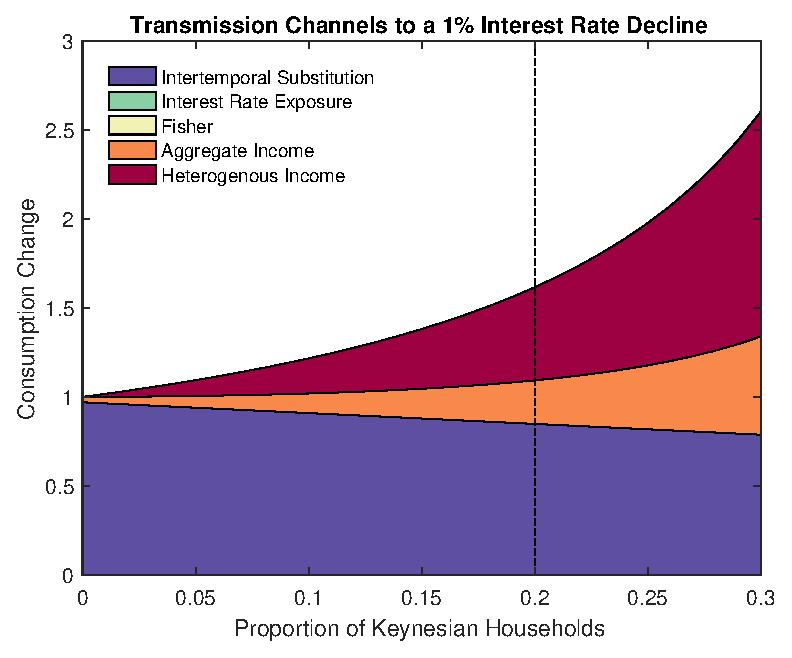
\includegraphics[scale=0.7]{../Matlab/DynareCode/Figures/ProportionKeynesian_sigma1.eps}
		\caption{Changing the Proportion of Keynesian Households, $\sigma=1$}
		\label{fig:ProportionKeynesian}
	\end{centering}
\end{figure}

This feature of the standard New Keynesian model, that markups are low during a boom and high during a recession, is not backed by empirical evidence and has led some away from price frictions and toward nominal wage frictions.\footnote{This point is emphasized in \cite{broer_2018} and motivates modeling choices in \cite{auclert_inequality_2018}}. While we are sympathetic to this approach, for this paper we maintain the sticky price assumption to stay close to the existing HANK literature. One way to remove this earnings heterogeneity channel completely would be to divide the income from capital and profits proportionally between the Keynesian and Ricardian households. In that model, the total consumption change would remain unchanged as the number of Keynesian households increased, with the intertemporal substitution channel decreases proportional to the share of Ricardian's in the economy and the aggregate income channel making up the remainder. While the channels would be different, in this model the aggregate dynamics would be \textit{identical} to the RANK model.

\subsection{Introducing Debt}
In this section we analyze what happens when the Keynesian households are allowed to take on debt equal to some fraction of their steady state income. For the remainder of this section we will fix the proportion of Keynesian households at 0.2, giving an economy-wide MPC of just over 20 percent. This number is chosen both because it is close to a number of the current theoretical HANK models, and a larger number causes indeterminacy problems for some parameterizations.\footnote{See \cite{gali_2004} for a detailed discussion on determinacy of TANK models.} However, we accept 0.2 is on the low end of empirical estimates.\footnote{A large literature aims to estimate MPCS. See \cite{johnson_household_2006}, \cite{parker_consumer_2013}, \cite{fagereng_mpc_2016} and \cite{ckConsumption} for a small selection of examples.} In figure \ref{fig:ProportionKeynesian} from the previous section, there is a dotted line drawn where the proportion of Keynesian households equals 0.2. This shows the size of the transmission channels for this section when there is no debt.

Figure \ref{fig:KeynesianDebt} shows how the size of the transmission channels change with the level of debt held by the Keynesian households, with the three panels showing this for decreasing elasticity of substitution.\footnote{The elasticity of substitution is equal to $1/\sigma$, so the three panels in figure \ref{fig:KeynesianDebt} represent an elasticity of substitution of 1, 0.5 and 0.33 respectively.} Starting with the left hand panel, we consider how the model behaves with an elasticity of substitution equal to one. The intercepts with the y-axis exactly correspond with the intercepts with the dotted line from figure \ref{fig:ProportionKeynesian}. This is the size of the transmission channels when a proportion 0.2 of households are Keynesian and these households have no debt. As in the previous section, the intertemporal substitution channel is slightly below one, while the income channels also play a significant role due to presence of Keynesian households. However, with no debt at the intersection with the y-axis both the interest rate exposure and Fisher channels are zero.

\begin{figure} 
	\begin{centering}
		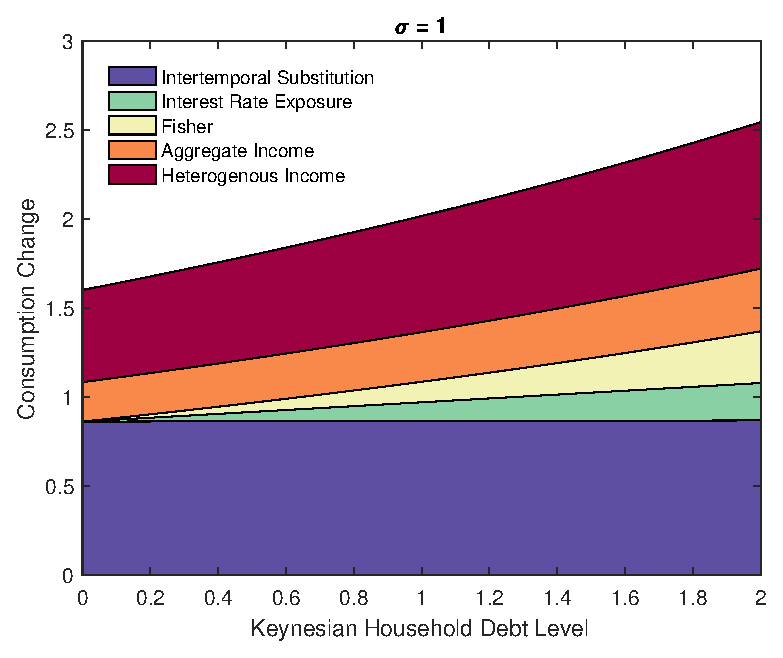
\includegraphics[scale=0.4]{../Matlab/DynareCode/Figures/KeynesianDebt_sigma1.eps}
		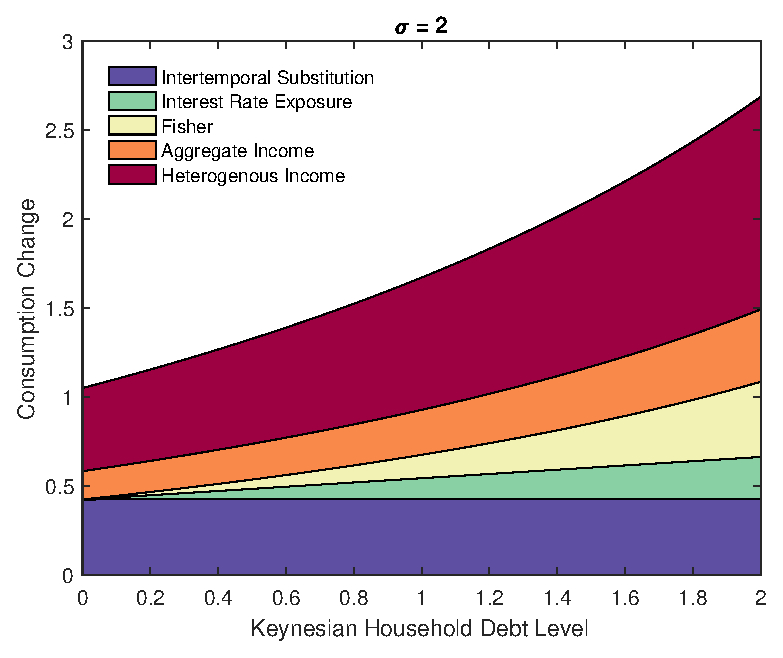
\includegraphics[scale=0.4]{../Matlab/DynareCode/Figures/KeynesianDebt_sigma2.eps}
		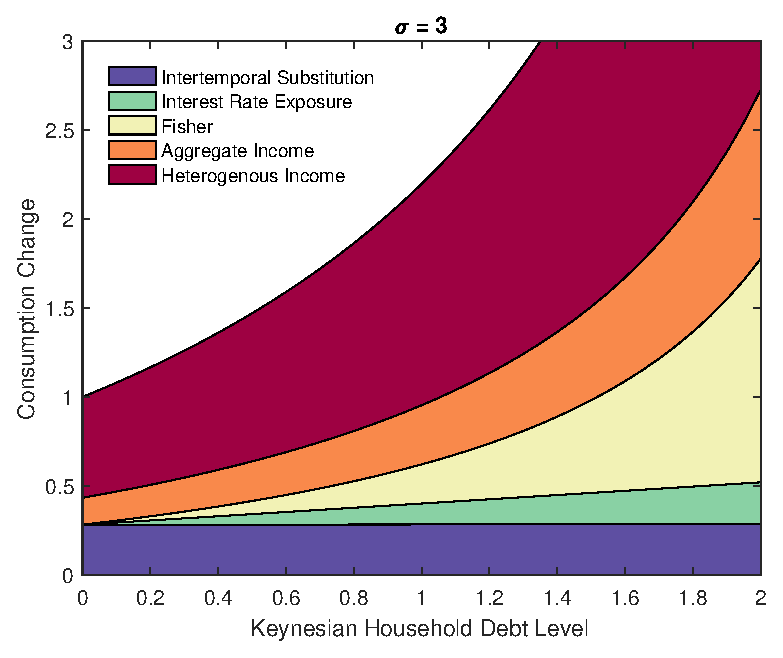
\includegraphics[scale=0.4]{../Matlab/DynareCode/Figures/KeynesianDebt_sigma3.eps}
		\caption{Changing the Debt of Keynesian Households}
		\label{fig:KeynesianDebt}
	\end{centering}
\end{figure}

As the quantity of debt that the Keynesian households can take on increases, both the interest rate exposure and Fisher channel start to become quantitatively important. Still looking at the left hand panel of figure \ref{fig:KeynesianDebt}, we see both of these channels growing, but they are still dominated by the intertemporal substitution channel. The two income channels grow in exact proportion to the other three channels, acting as a constant multiplier of the other three channels, no matter the quantity of debt. It may be useful to think of the transmission of monetary policy acting in stages. First aggregate demand is directly affected by the intertemporal substitution and interest rate exposure channels. The size of these channels depends only on the change in the interest rate, and is not changed as output and inflation change. The size of the Fisher channel is proportional to the amount of nominal debt, multiplied by the size of the overall change in income.\footnote{This is because inflation is proportional to the output gap in this model.} Finally the income channels are each a constant proportion of the total income change. We can think of intertemporal substitution and interest rate exposure as providing the initial `kick', which is then augmented by the Fisher and income channels.

The center and right panels of figure \ref{fig:KeynesianDebt} show the same channels, but when the elasticity of substitution is 0.5 and 0.33 respectively. The size of the intertemporal substitution channel is reduced in the same proportion, by 0.5 and 0.33 as the Ricardian households are now less happy to shift consumption between periods. However, the interest rate exposure channel remains exactly the same size as before. It is determined by the change in the borrowing cost along with the size of the debt, both of which are unchanged. The aggregate income channel is also exactly the same multiple of the other channels in all three panels, as is the Fisher channel.\footnote{The aggregate income multiplier is constant across both debt levels and intertemporal elasticity. The Fisher multiplier varies by debt level, but for any particular debt level it does not vary with intertemporal elasticity} The earnings heterogeneity multiplier grows significantly with $\sigma$. This is because the markup, and hence firm profits, become \textit{more} countercyclical with higher $\sigma$. Again, this feature of the standard New Keynesian model is undesirable and leads us here to be unable analyze the model under low elasticities of substitution that we believe to be more empirically reasonable.\footnote{See \cite{havranek_measuring_2015} for a meta-study for EIS estimates.}

This brings us to a broader point: the calibration of the elasticity of intertemporal substitution (EIS) in the standard New Keynsian model has been chosen to match aggregate data, despite the little micro evidence we have suggesting a much lower level. Figure \ref{fig:KeynesianDebt} shows why, in the absence of debt, a large EIS is required: with no debt the intertemporal substitution channel is the only `kick' to aggregate demand, so if this is small we need very large multipliers to get a sizable consumption response to monetary policy. If we make the EIS small, we need something else to take its place. Interest rate exposure is another `kick', that empirical evidence has shown could be large,\footnote{See \cite{auclert_monetary_2017} and \cite{ckConsumption}.}. By introducing interest rate exposure, we allow our models to use more micro-founded estimates of the EIS while still generating the kinds of aggregate responses estimated in the macro data.

\section{Relaxing the Fixed Capital Assumption}
Instead of a fixed amount of capital, K, allow for investment. If there are no costs to investment, then households will invest until the new capital stock gives risk to the changed interest rate, which will result in a very persistent change in the interest rate. We will need convex investment adjustment costs to avoid this persistence, and hope to show that reasonable calibrations result in little change in the capital stock and hence low interest rate persistence. Auclert did something like this in a previous version of his paper.

\subsection{The Model}
The model is identical to the baseline model, except for the fact that the Ricardian households are now able to invest in capital as well as nominal bonds. Aggregate investment at time $t$, $\text{Inv}_t$, along with the level of capital at time $t$, $K_t$, together determine the capital level at time $t+1$:
\begin{align}
\text{Inv}_t = \Phi\left(\frac{K_{t+1}}{K_t}\right) K_t
\end{align}
where $\Phi(1) =\delta$ is the per period depreciation, $\Phi'(1) =1$ and $\Phi''(1) =\psi_K >0 $ represents convex capital adjustment costs. It is the fact that capital in period $t+1$ is \textit{predetermined} in period $t$ that differentiates this model from the baseline model in terms of breaking the assumptions required for Auclert's decomposition to hold. In steady state the investment share of income is $\overline{\textit{inv}} = \frac{\varepsilon-1}{\varepsilon} \frac{\delta \alpha}{1/\beta - (1-\delta)}$.\footnote{This comes from equating the steady-state return from investment with $1/\beta$, the steady-state real interest rate, and using the fact that in equilibrium the total income allocated to capital is equal to $\frac{\alpha}{1-\alpha}$ times the total income allocated to labor. For other steady-state ratios, equation \ref{c_K_ss} remains the same, but now $\overline{c}_{R}=1-\overline{\textit{inv}}-\overline{c}_{K}$, taking account of the fact that investment now takes a chunk out of output which is no longer equal to aggregate consumption.}

\subsection{Changes Relative to the Linear Baseline Model}
Given nominal interest rate and inflation expectations, the individual optimization problems for both Ricardian and Keynesian households, as well as firms, remains identical to the baseline model. That results in equations \ref{euler_R_linear}, \ref{NKphillips_linear}, \ref{budget_constraint_K_linear}, and \ref{foc_hours_linear} remaining unchanged. Differences occur in aggregation.

As the natural level of output (output that would occur with flexible prices) is no longer constant, the output gap, $\tilde{y}$, is no longer equal to output. The model needs equations to define the natural level output and the output gap:\footnote{Natural output is derived from the fact that under flexible prices, the markup over marginal cost will be constant ($\frac{\varepsilon}{\varepsilon-1}$).}
\begin{align}
y^{n} &= \frac{\alpha(1+\psi)}{\sigma(1-\alpha) + \psi + \alpha} k_{t} \label{y_nat_linear} \\
\tilde{y}_t &= y_t - y^{n}	\label{output_gap_linear}
\end{align}
Furthermore, the aggregate production function, equation \ref{production_linear}, now includes capital:
\begin{align}
\tilde{y}_t &= \alpha k_t +  (1-\alpha)n_t  \label{production_capital_linear}
\end{align}
Aggregation of output now includes the investment share, so equation \ref{agg_C_linear} is replaced by:
\begin{align}
y_t &= \overline{c}_{K} c^K_t + \overline{c}_{R} c^R_t + \overline{\textit{inv}} \ \textit{inv}_t \label{agg_Y_linear}
\end{align}
The law of motion for capital is introduced to the model:
\begin{align}
\delta \ \textit{inv}_t = k_{t+1} - (1-\delta) k_{t}    \label{lom_capital}
\end{align}
As is the equation for the shadow price of capital, $q_t$, determined by the convexity of adjustment costs:
\begin{align}
q_t = \psi_K (k_{t+1}-k_t)	\label{shadow_K}
\end{align}
Finally we require an equation to equate the expected return on investment with the expected real return on nominal bonds:
\begin{align}
r_t + q_t = \beta (1-\delta) \mathbb{E}_t q_{t+1} + (1 - \beta (1-\delta)) (\mathbb{E}_t (w_{t+1} + n_{t+1}) - k_{t+1})	\label{return_K}
\end{align}

\subsection{Results from the Model with Investment}
For our partial equilibrium decomposition to approximate the aggregate consumption change, the shock to income, interest rates and inflation must be close to transitory. This poses a serious challenge for a model with capital, which is a slow moving variable. Figure \ref{fig:PathCap} shows the problem. The figure displays the path of capital following a one percentage point negative shock to the nominal interest rate for different levels of capital adjustment convexity. Immediately we can see capital is a very persistent variable, with more than half of the increase in capital still present after six years. When there is no convexity in the capital adjustment costs ($\psi_c = 0$), the one percentage point decrease in the nominal rate results in a \textit{large} positive increase in the quantity of capital. For typical values of $\psi_c$, often between one and three, the change is an order of magnitude smaller, while unsurprisingly capital remains unchanged in the case of infinite capital adjustment costs. This suggests the case of infinite adjustment costs will be similar to the fixed capital model. As we will see later this is mostly true, but the presence of positive investment makes the measurement of URE more subtle.

\begin{figure} 
	\begin{centering}
		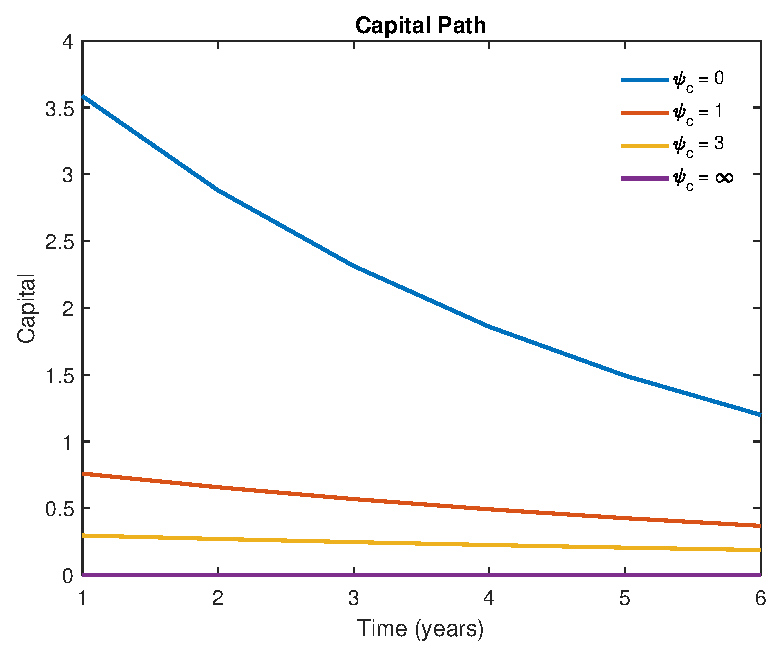
\includegraphics[scale=0.7]{../Matlab/DynareCode/Figures/TANK_capital_IRF_k.eps}
		\caption{Path of Capital following a 1\% nominal interest rate shock}
		\label{fig:PathCap}
	\end{centering}
\end{figure}

As figure \ref{fig:PathCap} makes clear, capital is highly persistent. However, we can see in figure \ref{fig:iandcpath} that in the cases where $\psi_c \geq 1$ the nominal interest rate path along with the consumption path for both Keynesian and Ricardian households is close to transitory. First consider the paths from figure \ref{fig:iandcpath} in which there are no convex adjustment costs to capital. In this case a one percent decrease in the nominal rate is highly persistent, as the level of capital fully adjusts such that the marginal product of capital is lower by the change in interest rate and this change in persists. All this extra investment in the first period dramatically (and unrealistically) increases wages, which the Keynesian households consume that period. Ricardian households invest most of their extra income, which allows them to maintain a higher path of consumption going forward.

When convex adjustment costs are introduced things look very different. Ricardian housesholds can no longer increase capital to maintain consumption going forward, because the adjustment costs kick in. As a result the change in nominal interest rate is almost entirely transitory (in the case where $\psi_c=\infty$ this is exactly true), as is the change in consumption behavior of both types of household. Again, due to the countercyclical behavior of profits in the standard New Keynesian model, Keynesians react much more to the change than Ricardians.

In order to quantify how large of a deviation the model with capital is from the assumptions needed for our decomposition to work exactly, table \ref{table:error} shows the percent difference between the true consumption change and that estimated using the partial equilibrium decomposition. The table shows the error for total consumption, as well as the error individually calculated for both the Ricardian and Keynesian households. First note that the method correctly estimates the consumption changes for the Keynesian households. This is because their behavior only depends on current income and the persistence can only affect consumption through the intertemporal substitution channel and wealth effects, which in their case are always zero. The error for Ricardian households (and overall consumption change) is unsurprisingly large when there are no convex adjustment costs, but this quickly comes down for standard calibrations if $\psi_c$ between 1 and 3. Furthermore, as the value of $\sigma$ rises, and the intertemporal substitution channel gets relatively smaller, this error diminishes.

\begin{figure} 
	\begin{centering}
		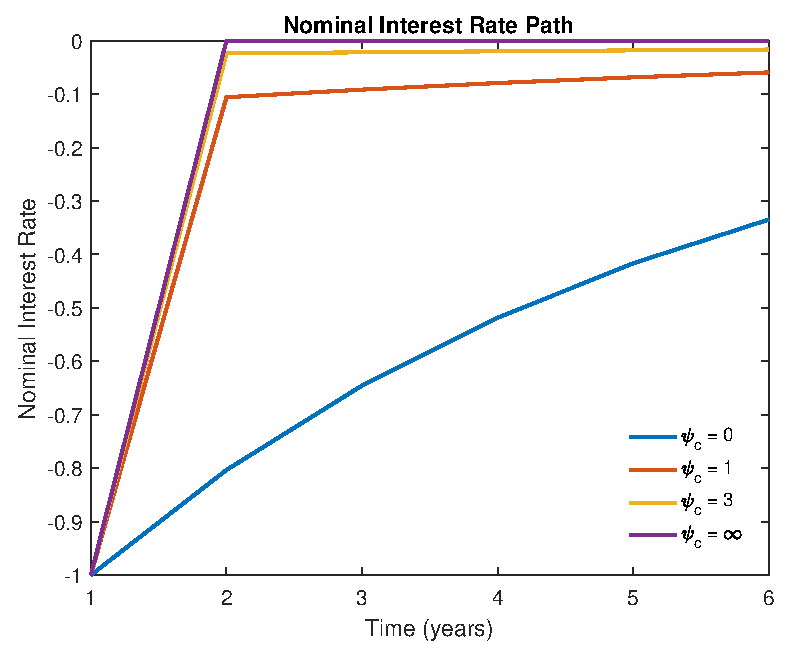
\includegraphics[scale=0.4]{../Matlab/DynareCode/Figures/TANK_capital_IRF_i.eps}
		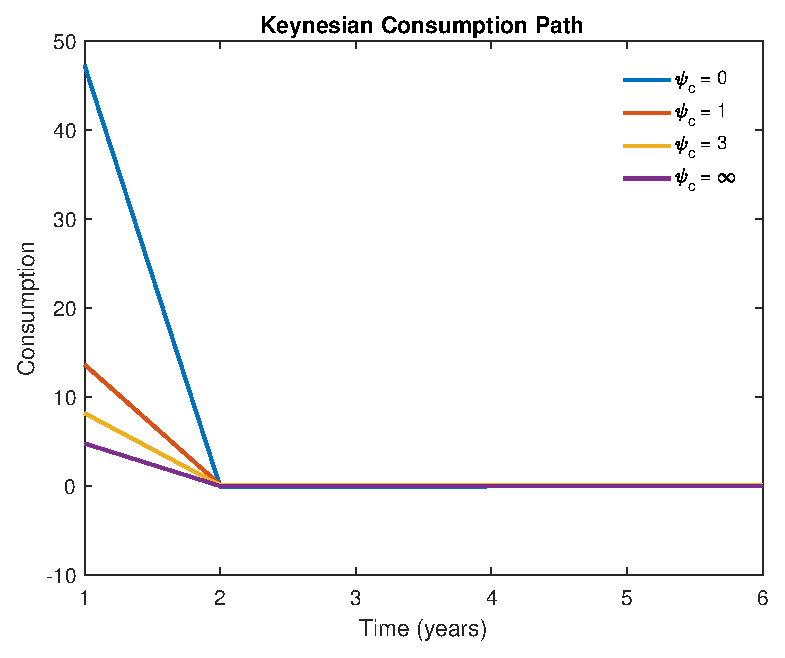
\includegraphics[scale=0.4]{../Matlab/DynareCode/Figures/TANK_capital_IRF_c_K.eps}
		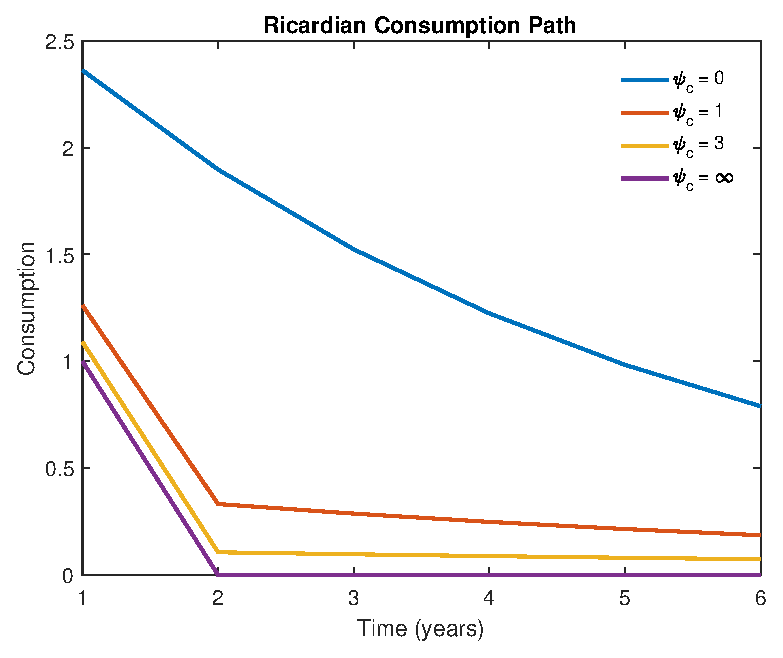
\includegraphics[scale=0.4]{../Matlab/DynareCode/Figures/TANK_capital_IRF_c_R.eps}
		\caption{Paths following a 1\% nominal interest rate decrease}
		\label{fig:iandcpath}
	\end{centering}
\end{figure}

The existence of capital raises the question of whether we should be including a wealth effect as a separate channel through which monetary policy operates. With convex capital adjustment costs, a decrease in the interest rate will increase the value of existing capital and hence the wealth of capital holders. Indeed this is also the case in the baseline fixed capital model. In that model the stream of income to the Ricardians from the capital is  offset by the stream of consumption generated by it. While the Ricardians increase their wealth when the price of capital increases, this is exactly offset by the increase in the value of their planned consumption. That is the increase in wealth does not allow them in increase their consumption in every period, it is instead an artifact of the fact that with a lower interest rate consumption today is relatively cheaper, that is the wealth effect is entirely subsumed in the intertemporal substitution effect.

The model with capital does not allow such an easy interpretation of the change in wealth, even in the case with infinite capital adjustment costs. This is because the Ricardians are consistently investing to offset depreciation. In our decomposition this saving counts as unhedged interest rate exposure because their return on investment will be equal to the real interest rate. However, investments that were already planned will not be subject to this higher price - it is the marginal investments that suffer from the convex adjustment costs. If we change our definition of unhedged interest rate exposure to exclude planned investment, then partial equilibrium decomposition gives no error for the model with infinite adjustment costs.

\input ../Matlab/DynareCode//Tables/error_table.tex

The change in the value of existing assets is shown in figure \ref{fig:PathTobinq}. With no adjustment costs the value of assets remains constant over time as the consumption asset is freely exchangeable with capital next period. Similarly, with infinite adjustment costs the price of a unit of capital next period moves one for one with the interest rate. For values in between the price of assets jumps up in period one followed by a persistent period in which capital adjusts back down to the steady state, and hence assets prices also low due to convex adjustment costs.

Overall the partial equilibrium decomposition works reasonably well with the addition of capital in the TANK model. However, in our model firms are risk neutral and it is clear that models in which firms are also able to have unhedged exposures to inflation and interest rates could complicate the transmission mechanism in quantitatively important ways. This may be especially true with the introduction of the banking sector, which has been shown emprirically to hold large unhedged interest rate exposures./footnote{See \cite{landier_banks_2013}. While empirical evidence suggests households are negatively exposed to interest rate hikes, the financial sector seems to be positively exposed. This suggests the transmission of monetary policy may be very different in times when the banking sector is working well to those when the banking sector is in crisis (when interest rate declines may not be as effective).}

\begin{figure} 
	\begin{centering}
		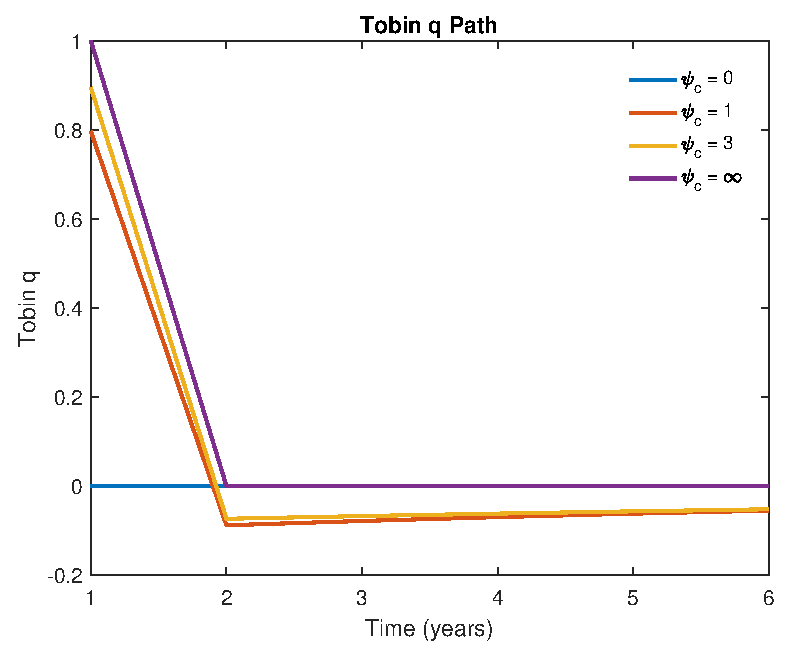
\includegraphics[scale=0.7]{../Matlab/DynareCode/Figures/TANK_capital_IRF_q.eps}
		\caption{Path of Tabin's q following a 1\% nominal interest rate shock}
		\label{fig:PathTobinq}
	\end{centering}
\end{figure}

\section{A Simple HANK Model}

\subsection{The Model}
The model we study is a one asset version of the HANK model presented in \cite{blSolving}. We also follow the solution method presented in that paper.

\subsubsection{Households}
In a given period household $i$ has labor productivity $h_{it}$, chooses their consumption $c_{it}$ and hours worked $n_{it}$. Households have Greenwood, Hercowitz and Huffman (GHH) preferences and act in order to maximize their expected utility:\footnote{The use of GHH preferences is primarily motivated to significantly simplify the solution method. \cite{arGHH} show GHH preferences can lead to unrealistically large fiscal multipliers, while separable preferences lead to other counter factual results.}
\begin{align*}
\mathbb{E} \sum_{t=0}^{\infty}\beta^t  u(c_{it} - \nu(n_{it} h_{it})) 
\end{align*}
where $u(x) = \frac{x^{1-\sigma}}{1-\sigma}$ and $\nu(n) = \frac{x^{1-\psi}}{1-\psi}$.

Households consume a consumption bundle formed according to a Dixit-Stiglitz aggregator:
\begin{align*}
c_{it} = \left(\int_{j=0}^{1} c_{ijt}^{\frac{\varepsilon-1}{\varepsilon}} dj \right)^{\frac{\varepsilon}{\varepsilon-1}}
\end{align*}
The price of each good is $p_{jt}$ resulting in the aggregate price level $P_t = \left(\int_{j=0}^{1} p_{jt}^{1-\varepsilon} dj \right)^{\frac{1}{1-\varepsilon}}$ with demand for each good:
\begin{align*}
c_{ijt} = \left(\frac{p_{jt}}{P_t} \right)^{-\varepsilon} c_{it}
\end{align*}

Household labor productivity evolves according to a $\log-AR(1)$ process, with a fixed probability that the household becomes an entrepreneur, receives no labor income, but instead collects a share of the firm profits:
\begin{align*}
h_{it} = \begin{cases}
				\exp(\rho_h h_{it-1} + \epsilon^h_{it}) &\text{ with prob } 1-\zeta \text{ if } h_{it-1} \ne 0\\
				0 &\text{  with prob } \iota \text{ if } h_{it-1} = 0 \\
				1	&\text{ otherwise}
\end{cases}
\end{align*}
That is a non-entrepreneur switches to an entrepreneur state with probability $\zeta$, while an entrepreneur switches to a non-entrepreneur with unit labor productivity with probability $\iota$. All households choose the same number of hours, due to GHH preferences. Total productive hours worked, $\int_{i=0}^{\infty} h_{it}n_{it}di = N(\omega_t)$, therefore depend only on the real wage, $\omega_t$.

In the entrepreneur state the household receives a fixed share of the economic profits of the firms, $\Pi_t$, and these rents are not tradeable.

Households must pay a tax $\tau$ on all their rent and labor income.

\subsubsection{Price Setting}
Prices are set by risk-neutral managers who form a group of measure zero.\footnote{Assuming the price setters are risk neutral makes the optimal price setting problem tractable without taking away from the important economics of the model.} We assume \cite{rotemberg_sticky_1982} pricing frictions, leading to a New Keynesian Phillips curve:
\begin{align*}
\log\left(\frac{P_t}{P_{t-1}}\right) = \beta \mathbb{E}_t \left( \log \left(\frac{P_{t+1}}{P_{t}}\right) \frac{Y_{t+1}}{Y_{t}} \right) + \kappa \left( MC_t - \frac{\varepsilon-1}{\varepsilon} \right)
\end{align*}
where $Y_t$ is total output in period $t$, $MC_t$ is the real marginal cost and $\kappa$ measures the size of the Rotemberg price frictions. In equilibrium all goods will have the same price.

\subsubsection{Fiscal Policy}


\subsubsection{Monetary Policy}
As in the TANK model, we assume the central bank follows the Taylor rule given in equation \ref{taylor_rule}.

\subsection{Results from the HANK model}


\section{Conclusion}
Lots of future research to do!


%\processdelayedfloats

\small
\bibliography{AllPapers}
\normalsize

\end{document}









